\documentclass[a4paper,12pt]{article}

\usepackage{graphicx}
\usepackage{wrapfig}
\usepackage{bidi}
\begin{document}
\section{LTR}
\subsection*{Wrapfig test}

Gulls are birds in the family Laridae. They are most closely
 related to the terns (family Sternidae), auks and skimmers,
and more distantly to the waders. Most gulls belong to the
large genus Larus.

\begin{wrapfigure}{r}{0.5\textwidth}
  \begin{center}
    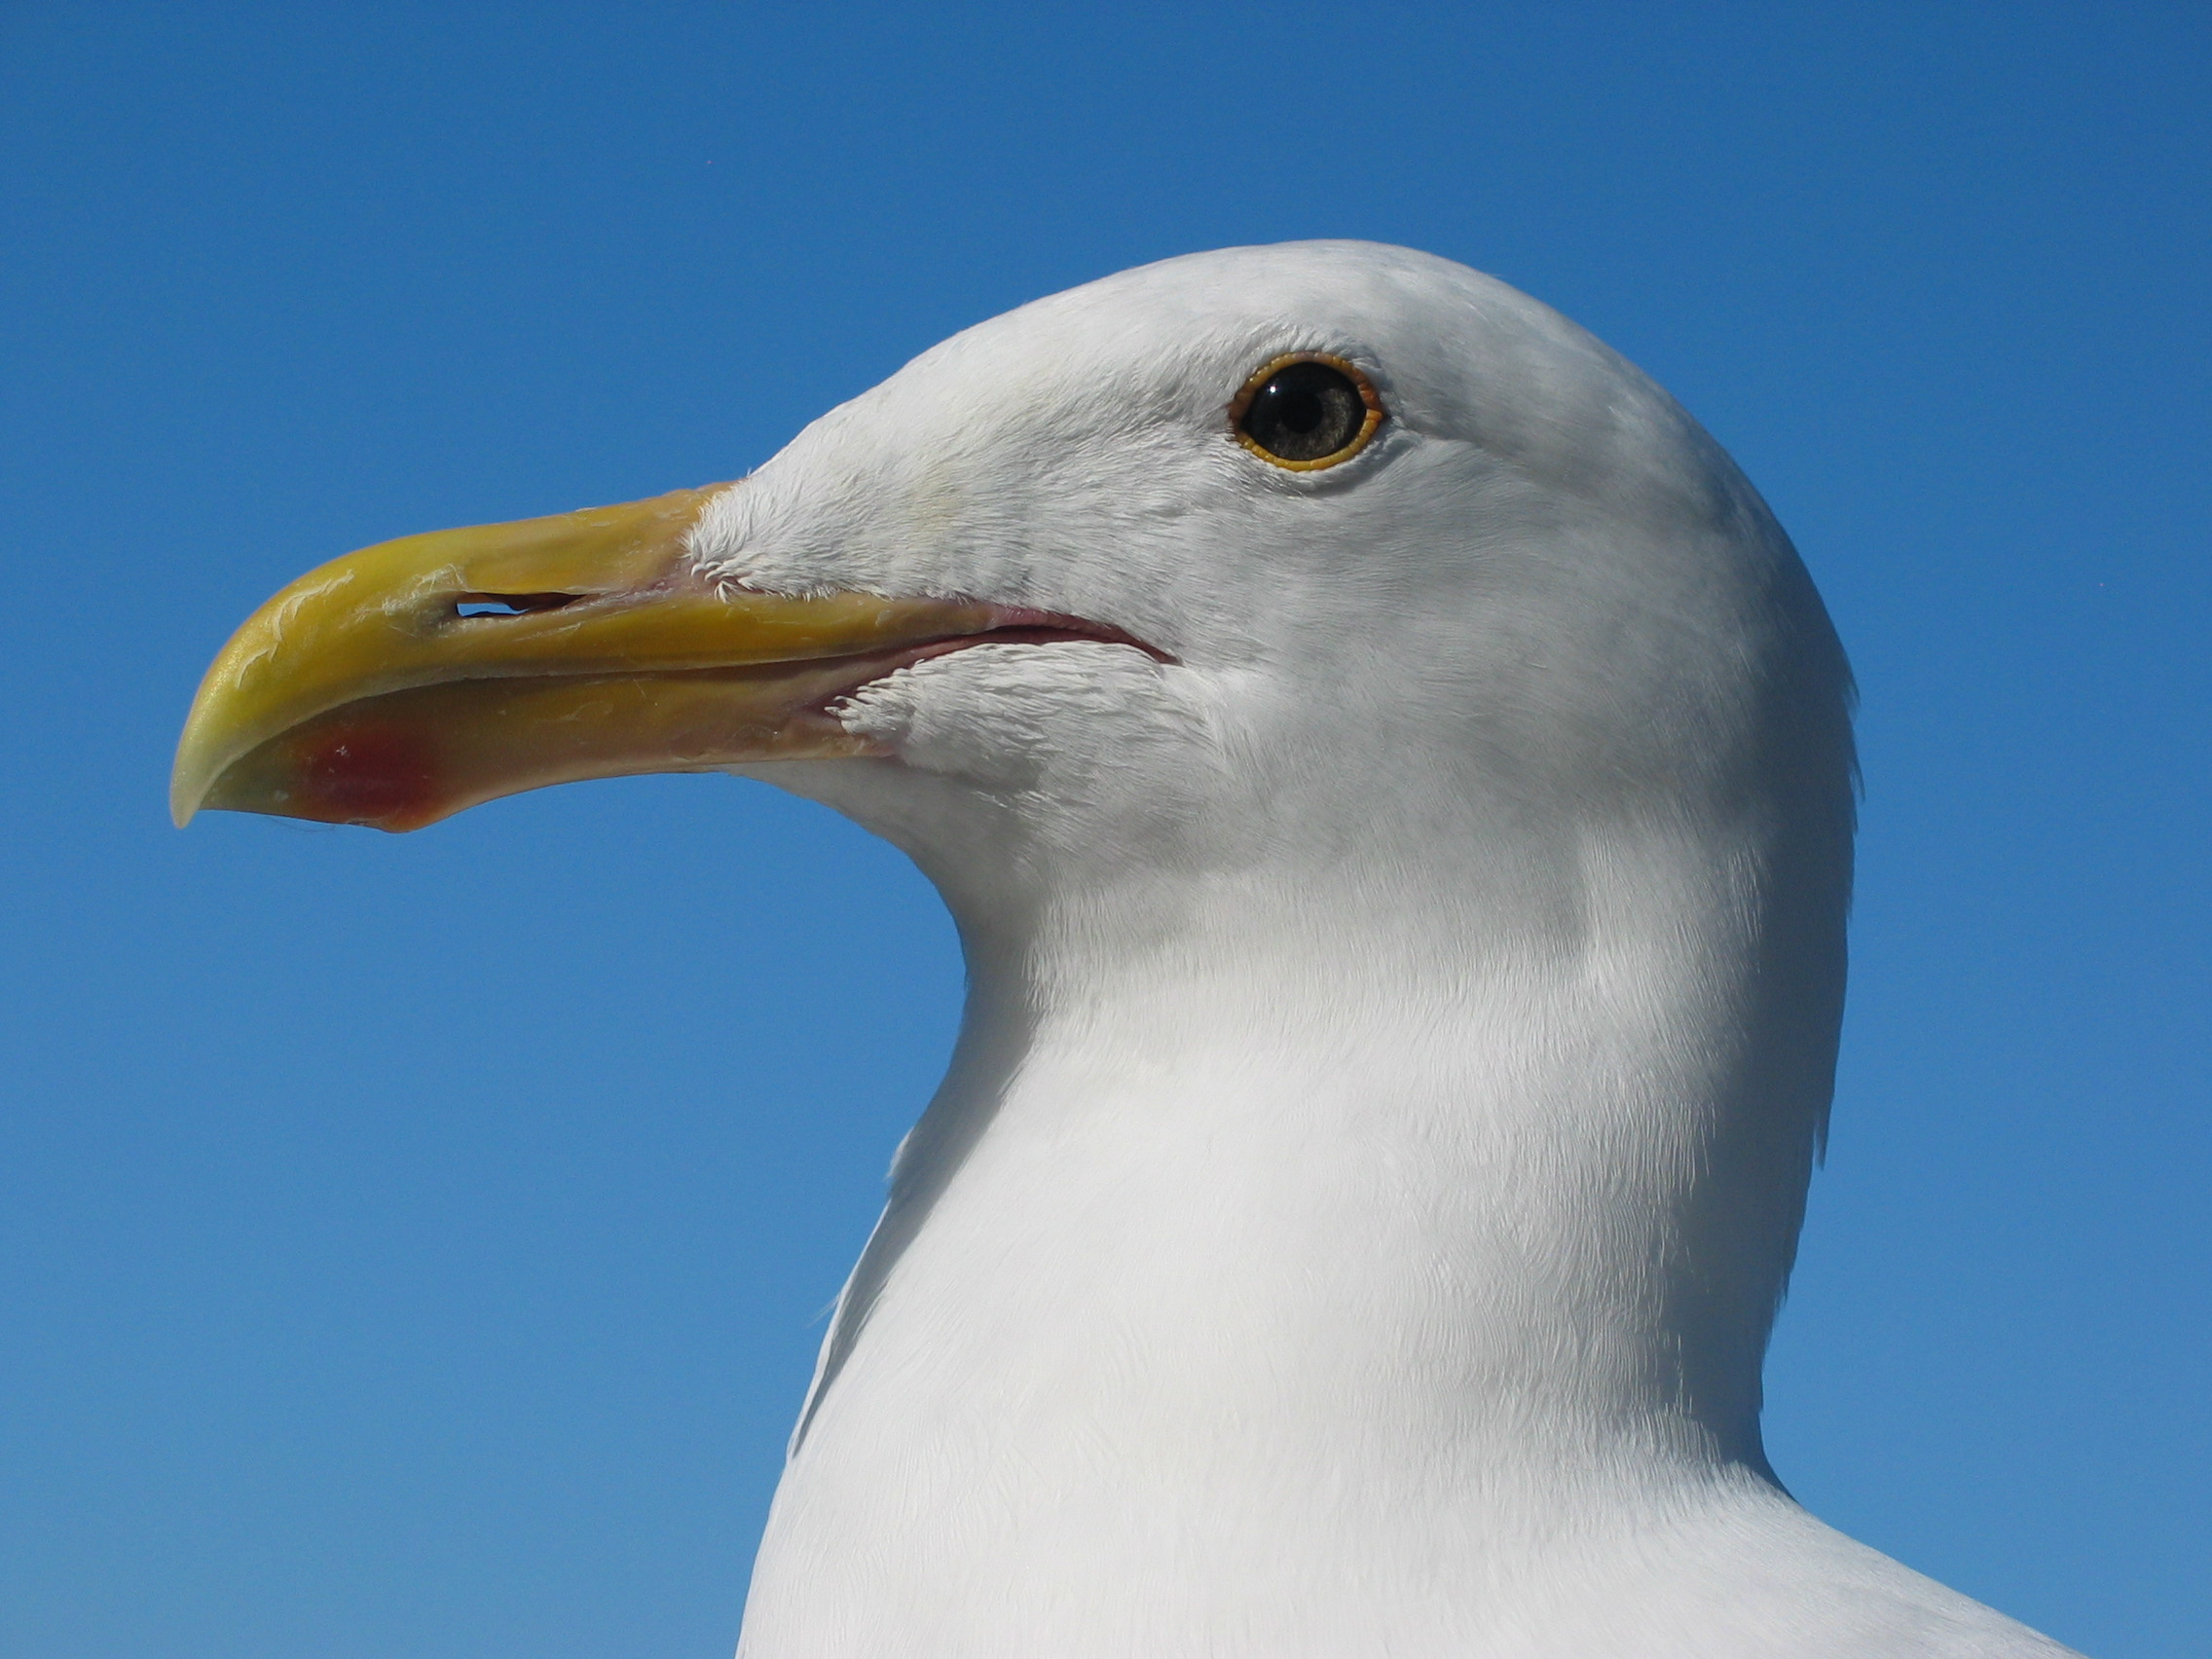
\includegraphics[width=0.48\textwidth]{gull}
  \end{center}
  \caption{A gull}
\end{wrapfigure}

They are in general medium to large birds, typically grey or white,
often with black markings on the head or wings. They have stout,
longish bills and webbed feet.

Most gulls, particularly Larus species, are ground nesting carnivores,
which will take live food or scavenge opportunistically. The live food
often includes crabs and small fish. Apart from the kittiwakes, gulls
are typically coastal or inland species, rarely venturing far out to sea.
The large species take up to four years to attain full adult plumage,
but two years is typical for small gulls.

Gulls---the larger species in particular---are resourceful and
highly intelligent birds, demonstrating complex methods of communication
and a highly developed social structure. Certain species (e.g. the
Herring Gull) have exhibited tool use behaviour. Many species of gull have
learned to co-exist successfully with man and have thrived in human habitats.
Others rely on kleptoparasitism to get their food.

\newpage
\section{RTL}

\setRTL
\subsection*{Wrapfig test}

Gulls are birds in the family Laridae. They are most closely
 related to the terns (family Sternidae), auks and skimmers,
and more distantly to the waders. Most gulls belong to the
large genus Larus.

\begin{wrapfigure}{l}{0.5\textwidth}
  \begin{center}
    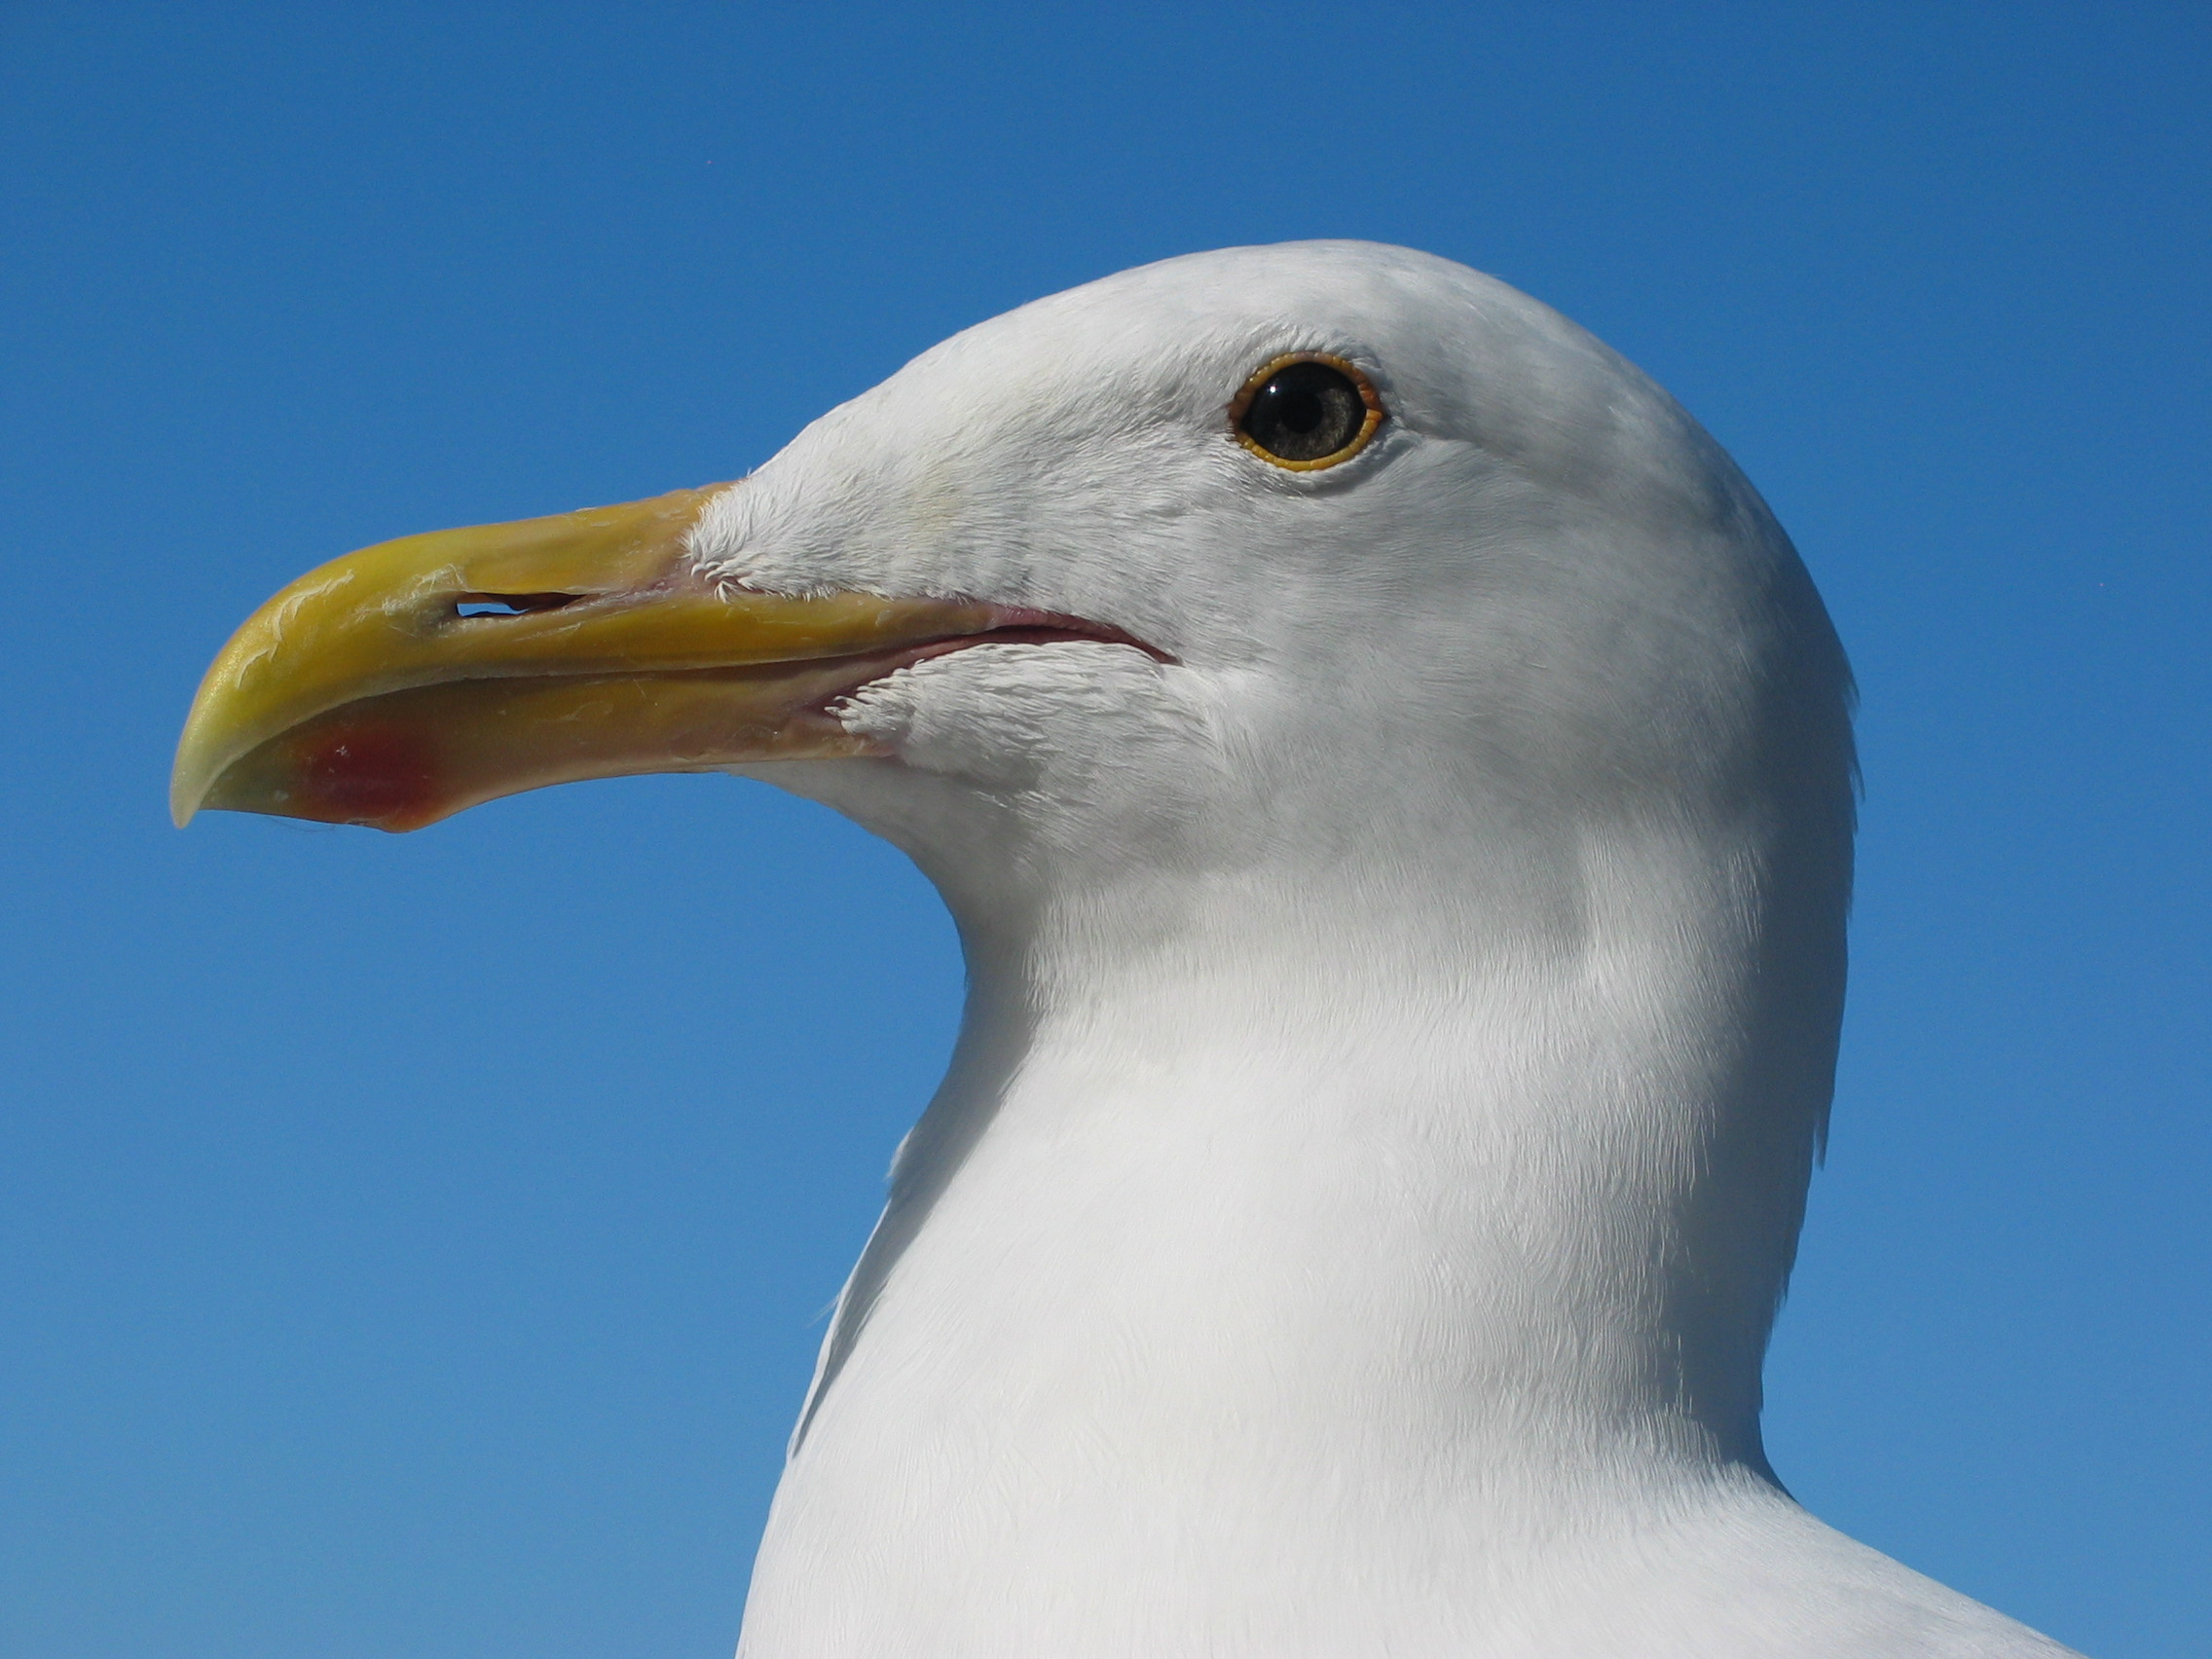
\includegraphics[width=0.48\textwidth]{gull}
  \end{center}
  \caption{A gull}
\end{wrapfigure}

They are in general medium to large birds, typically grey or white,
often with black markings on the head or wings. They have stout,
longish bills and webbed feet.

Most gulls, particularly Larus species, are ground nesting carnivores,
which will take live food or scavenge opportunistically. The live food
often includes crabs and small fish. Apart from the kittiwakes, gulls
are typically coastal or inland species, rarely venturing far out to sea.
The large species take up to four years to attain full adult plumage,
but two years is typical for small gulls.

Gulls---the larger species in particular---are resourceful and
highly intelligent birds, demonstrating complex methods of communication
and a highly developed social structure. Certain species (e.g. the
Herring Gull) have exhibited tool use behaviour. Many species of gull have
learned to co-exist successfully with man and have thrived in human habitats.
Others rely on kleptoparasitism to get their food.
\end{document}
